\documentclass[conference]{IEEEtran}
\IEEEoverridecommandlockouts
\usepackage{cite}
\usepackage{amsmath,amssymb,amsfonts}
\usepackage{algorithmic}
\usepackage{graphicx}
\usepackage{textcomp}
\usepackage{xcolor}
\usepackage[english,brazilian]{babel}
\usepackage[utf8]{inputenc}
\usepackage[T1]{fontenc}
\def\BibTeX{{\rm B\kern-.05em{\sc i\kern-.025em b}\kern-.08em
    T\kern-.1667em\lower.7ex\hbox{E}\kern-.125emX}}
\begin{document}

\title{Aplicando Técnicas de Mineração de Dados no Sistemas de Recomendação de Candidatos para Vagas de Emprego}

\author{
    \IEEEauthorblockN{ Bruno Lopes}
    \IEEEauthorblockA{
        \textit{bruno.lopes.ti@icloud.com}
    }
    \and
}
\maketitle

\begin{abstract}
%  1) contexto: identificar a grande area
%  2) nessa grande area precisa de pesquisar problemas em aberto
%  3) o que foi feito (objetivo)
%  4) metodologia: falar dos metodos utilizados
%  5) resultados: principal resultado
%  6)conclusao: como pode contruibuir para area de pesquisa
O volume de dados pode dificulta o processo de busca e filtragem de informação.  Quando se deseja buscar candidatos para preencher vagas, muitos recrutadores precisam analisar montantes de currículos, fazendo com que esse processo seja demorado. Com isso, sistemas de recomendação pode se tornar uma importante ferramenta para auxiliar os usuários nessa procura. Empresas como LinkedIn que trabalham com candidatos e vagas, já deram sua contribuição cientifica, e esse experimento foi baseado em um dos trabalhos publicados por Fedor Borisyuk, Krishnaram Kenthapadi, David Stein e Bo Zhao. Com base nos estudos realizados, foi desenvolvido uma rede neural artificial capas de classificar candidatos como aprovados ou reprovados. Foram aplicados processos de Mineração de Dados como pré-processamento, criação de \textit{bag of words } com TF-IDF para treinamento criação do modelo preditivo. O processo proposto aqui para desenvolvimento de um classificador capaz de recomendar candidatos pode otimizar muito o tempo de recrutadores.
\end{abstract}

\begin{IEEEkeywords}
Sistemas de Recomendação de Candidatos; Redes Neurais Artificiais; Mineração de Dados
\end{IEEEkeywords}
\selectlanguage{english}
\begin{abstract}
The volume of data can make it difficult to process and filter information. When it is desired to search for candidates to fill vacancies, many recruiters need to reduce amounts of resumes, making this process time-consuming. With this, recommendation systems can be an important tool to help users search. Companies like LinkedIn that work with candidates and vacancies, have already made their scientific contribution, and this experiment was based on one of the works published byFedor Borisyuk, Krishnaram Kenthapadi, David Stein and Bo Zhao. Based on the studies carried out, an artificial redeneural layer was developed to classify candidates as approved or disapproved. Data Mining processes were applied as pre-processing, creation of debug of words with TF-IDF for training creation of the predictive model. The process here proposed for the development of a candidate classifier to recommend candidates can greatly optimize the time workers.

\end{abstract}
\selectlanguage{brazilian}
\begin{IEEEkeywords}

Candidate Recommendation System; Artificial Neural Network; data mining
\end{IEEEkeywords}

\section{INTRODUÇÃO}

    

\section{Referencial Teórico}
	%Problema, base conceitual para a solução %
	
    A base de dados foi fornecida pela Reachr Soluções Inovadoras em RH, uma empresa privada que provê soluções digitais para todo processo de recrutamento e seleção de candidatos para corporações. Em cima desse conjunto conjunto de dados foram aplicados vários processos de Mineração de dados afim de extrais informações uteis para o negocio e além da aplicação de modelos preditivos utilizando técnicas de aprendizagem de máquina.
    	
    O modelo aplicado nesse experimento utiliza um Rede Neural Artificial(RNA)  a fim classificar quais candidatos serão ou não indicados para determinada vaga de trabalho. 
    	
    Redes neurais artificiais(RNA) são modelos inspirados na arquitetura neural do cérebro e foi desenvolvido para tentar modelar a capacidade de aprendizagem de sistemas neurais biológicos \cite{b4}. 
	
	\subsection{Mineração de dados}
	
	A mineração de dados é parte integrante do processo de descoberta de conhecimento em bases de dados (\textit{Knowledge Discovery in Databases}, ou KDD) \cite{mineracao_nunes}.
	
	Na primeira  conferência internacional sobre KDD realizada em 1995, foi dada uma definição para cada um dos termos, pois muitos autores consideravam os termos KDD e Data Mining como sinônimos \cite{mineracao_nunes}. 
    
    Segundo FAYYAD \cite{kdd}, o termo Knowledge Discovery in Databases ou KDD foi criado em 1989 como referência ao processo amplo de encontrar conhecimento em dados e dar ênfase a uma grande aplicação em particular - o método \textit{Data Mining }(Mineração de Dados).
    
    KDD refere-se a todo processo de descoberta de conhecimento útil de dados, enquanto a Mineração de Dados a uma das atividades do processo. Na figura 1 podemos ver uma representação do processo de KDD.
   
	\begin{figure}[htbp]
	\centerline{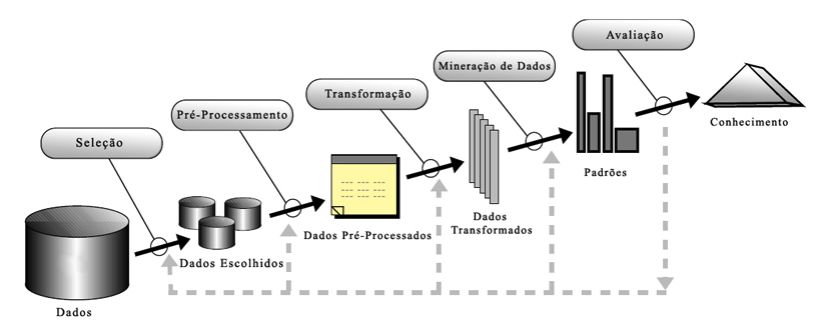
\includegraphics[scale=0.3]{imagens/kdd.png}}
	\caption{Uma visão geral das etapas que compõem o processo do KDD}
	
	\label{fig}
	\end{figure}

    Utilizamos para o experimento alguns processos de Mineração de Dados como: Estatística, Aprendizado de Máquina, Banco de Dados e Visualização. Dentre os quais foram aplicados pré-processamento, análise descritiva, classificação, detecção de anomalias entre outros.

    \subsection{Base de dados}

 O banco de dados utilizado nesse experimento foi provido pela Reachr Soluções Inovadoras em RH.
A base de dados foi extraída de um sistema gerenciador de banco de dados NoSQL ( bancos de dados não relacionais) cujo documento tinha o tamanho de 12,23 \textit{gigabyte} e continha 19 \textit{collections} (documentos) conforme descrito abaixo:

\begin{itemize}
\item DadosBasicos: dados básicos dos candidatos;
\item ExperienciaProfissional: experiencias profissionais dos candidatos;
\item FormacaoAcademica: formação acadêmica ensino médio, técnico, superior e etc;
\item Remuneracao: ultima remuneração;
\item Idioma; curso de idiomas com seu respectivo nível;
\item DadosComerciais; dados de empresas ;
\item detalhesempresa; dados detalhados de empresas
\item vaga: dados das vagas oferecidas;
\item OutrasInformacoesEstagio: afirmações especificas para candidatos que busquem estagio
\item Empresa: dados de empresas;
\item Indicacao: indicação de candidato para candidato
\item OutrasInformacoesGerente: 
\item PPI: \textit{ranking} criado pela empresa para posicionar candidatos;
\item RemuneracaoPart: ultima remuneração;
\item Empregabilidade: índice de empregabilidade criado com regras próprias;
\item MatchPart: indica a qual vaga o candito esta e em qual etapa
\item Estatisticaestágio: dados criados para criar um \textit{ranking} dos estagiários
\item Estatisticacomercial: dados comerciais de cada empresa;
\item Etapas: etapas customizadas pela empresa;
\end{itemize}

Durante a etapa de pre-processamento muitos dos documentos não tiveram relevância para nossa análise e foram removidos,

	\subsection{Pré-processamento de dados}
  O processo de preparação dos dados para a mineração, também chamado de pré-processamento, segundo Han e Kamber \cite{mineracao_conceitos_tecnicas}, tem função de aprimorar a qualidade dos dados fazendo com que os processos de Mineração de dados fiquem mais eficientes.
 
    Os dados têm qualidade se satisfizerem os requisitos do uso pretendido . Há muitos factores que compreendem a qualidade dos dados, incluindo exatidão, integridade, consistência, oportunidade, credibilidade e interpretabilidade\cite{mineracao_conceitos_tecnicas}.
      
     Não se pode esperar que bases de dados não tenha problemas pertinentes a erro humano, falhas na coleta ou problemas com dispositivos de medição. Dados do mundo real tendem a ser incompletos, ruidosos e inconsistentes \cite{mineracao_conceitos_tecnicas}. 

    Podemos ver na  Figura 2 uma visão do processo de preparação da base de dados.

\begin{figure}[htbp]
	\centerline{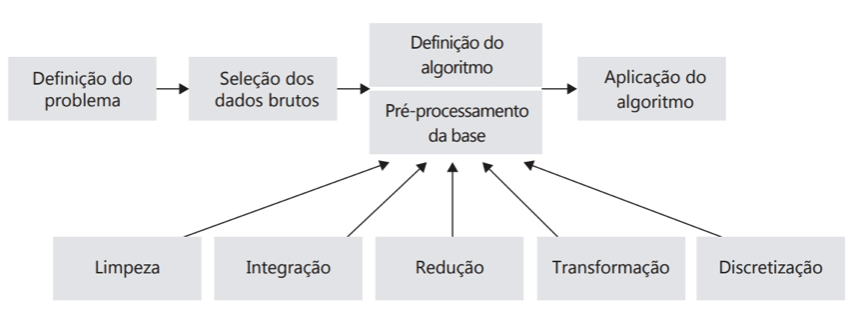
\includegraphics[scale=0.3]{imagens/preprocessamento.png}}
	\caption{Etapas do processo de preparação da base}
	
	\label{fig}
	\end{figure}

As principais tarefas de pré-processamento são  \cite{mineracao_nunes}:
\begin{itemize}
\item Limpeza: para imputação de valores ausentes, remoção de ruídos e correção de inconsistências;
\item Integração: para unir dados de múltiplas fontes em um único local, como um armazém de dados;
\item Redução: para reduzir a dimensão da base de dados;
\item Transformação: para padronizar e deixar os dados em um formato passível de aplicação das diferentes técnicas de mineração;
\item Discretização: transforma atributos contínuos em atributos categóricos;
\end{itemize}

Durante a etapa de pré-processamento, conseguiu-se reduzir dimensionalidade e selecionar somente os dados apresentados nas Tabelas I e II para criar nosso sistema de recomendação. Lembrando que os mesmos foram extraídos dos seguintes documentos: 
\begin{enumerate}
\item ExperienciaProfissional
\item Vaga
\item DadosBasicos
\item FormacaoAcademica
								
\begin{table}[h]
 \centering
% distancia entre a linha e o texto
 {\renewcommand\arraystretch{1.25}
\caption{Representação estruturada de um perfil de candidato}
 \begin{tabular}{ l l }
  \cline{1-1}\cline{2-2}  
    \multicolumn{1}{|p{3.0cm}|}{\cellcolor{}Campo \centering } &
    \multicolumn{1}{p{4.217cm}|}{\cellcolor{}Valor do campo \centering }
  \\  
  \cline{1-1}\cline{2-2}  
    \multicolumn{1}{|p{3.0cm}|}{Atividade profissional } &
    \multicolumn{1}{p{4.217cm}|}{ Líder técnico de desenvolvimento}
  \\  
  \cline{1-1}\cline{2-2}  
    \multicolumn{1}{|p{3.0cm}|}{  Cargo profissional } &
    \multicolumn{1}{p{4.217cm}|}{ Desenvolvedor Java Sênior}
  \\  
  \cline{1-1}\cline{2-2}  
    \multicolumn{1}{|p{3.0cm}|}{  Curso técnico} &
    \multicolumn{1}{p{4.217cm}|}{Técnico em informática }
  \\  
  \cline{1-1}\cline{2-2}  
    \multicolumn{1}{|p{3.0cm}|}{  Superior} &
    \multicolumn{1}{p{4.217cm}|}{ Ciências da Computação }
  \\  
  \cline{1-1}\cline{2-2}  
    \multicolumn{1}{|p{3.0cm}|}{  Pós-graduação} &
    \multicolumn{1}{p{4.217cm}|}{ Inteligencia Artificial}
  \\  
  \cline{1-1}\cline{2-2}  
    \multicolumn{1}{|p{3.0cm}|}{  Conhecimentos } &
    \multicolumn{1}{p{4.217cm}|}{ C++, Java, Linux, Aprendizado de Máquina }
  \\  
  \hline
 \end{tabular} }
\end{table}

\begin{table}[h]
 \centering
% distancia entre a linha e o texto
 {\renewcommand\arraystretch{1.25}
\caption{Representação estruturada de uma vaga}
 \begin{tabular}{ l l }
  \cline{1-1}\cline{2-2}  
    \multicolumn{1}{|p{3.0cm}|}{\cellcolor{}Campo \centering } &
    \multicolumn{1}{p{4.217cm}|}{\cellcolor{}Valor do campo \centering }
  \\  
  \cline{1-1}\cline{2-2}  
    \multicolumn{1}{|p{3.0cm}|}{Titulo} &
    \multicolumn{1}{p{4.217cm}|}{ Analista desenvolvedor Python}
  \\  
  \cline{1-1}\cline{2-2}  
    \multicolumn{1}{|p{3.0cm}|}{  Escolaridade desejada } &
    \multicolumn{1}{p{4.217cm}|}{Superior}
  \\  
  \cline{1-1}\cline{2-2}  
    \multicolumn{1}{|p{3.0cm}|}{  Descrição} &
    \multicolumn{1}{p{4.217cm}|}{ Construir aplicações utilizando }
  \\  
  \cline{1-1}\cline{2-2}  
    \multicolumn{1}{|p{3.0cm}|}{  Requisitos obrigatórios } &
    \multicolumn{1}{p{4.217cm}|}{ 4 anos de experiencia com Python, Serverless, Cloud e etc}
  \\  
  \cline{1-1}\cline{2-2}  
    \multicolumn{1}{|p{3.0cm}|}{  Conhecimentos desejados} &
    \multicolumn{1}{p{4.217cm}|}{ MongoDB, GIT, GIT Flow, Unix, REST API}
  \\  
  \hline
 \end{tabular} }
\end{table}


\end{enumerate}


Uma das tarefas que utilizamos para prepara os dados foi a tokenização que tem como objetivo dividir o texto em unidades conhecidas como \textit{tokens}. Essas unidades podem ser números, espaços, palavras ou termos compostos por mais de uma palavra. O processo de tokenização é feito, em geral, identificando-se espaços em branco e pontuações que costumam delimitar os termos \cite{tokenizacao}.

Depois de marcados estes termos, foram aplicadas técnicas de remoção de espaços em branco, a transformação de letras maiúsculas para minúscula, a retirada de números e de pontuação, remoção de palavras com pouco sentido semântico como artigos, preposições, conjunções, bem como outras palavras auxiliares que não agregam valor ao texto. Ex (de, a, o, que, e, do, da, em, um, para, com, não, uma, os, no, se, na) .
Para exemplificar melhor veja uma amostra com um dados real na Tabela III com valores originais e alterados.

\begin{table}[h]
 \centering
% distancia entre a linha e o texto
 {\renewcommand\arraystretch{1.25}
\caption{Aplicação ferramentas de limpeza de dados}
 \begin{tabular}{ l l }
  \cline{1-1}\cline{2-2}  
    \multicolumn{1}{|p{3.5cm}|}{\cellcolor{}Valor original \centering } &
    \multicolumn{1}{p{3.5cm}|}{\cellcolor{}Valor alterado \centering }
  \\  
  \cline{1-1}\cline{2-2}  
    \multicolumn{1}{|p{3.0cm}|}{Líder técnico de desenvolvimento } &
    \multicolumn{1}{p{4.217cm}|}{ lider tecnico desenvolvimento}
  \\  
  \cline{1-1}\cline{2-2}  
    \multicolumn{1}{|p{3.0cm}|}{  Desenvolvedor Java Sênior } &
    \multicolumn{1}{p{4.217cm}|}{ desenvolvedor java senior}
  \\  
  \cline{1-1}\cline{2-2}  
    \multicolumn{1}{|p{3.0cm}|}{ Técnico em informática } &
    \multicolumn{1}{p{4.217cm}|}{ tecnico informatica}
  \\  
  \cline{1-1}\cline{2-2}  
    \multicolumn{1}{|p{3.0cm}|}{  Ciências da Computação} &
    \multicolumn{1}{p{4.217cm}|}{ ciencias computacao }
  \\  
  \cline{1-1}\cline{2-2}  
    \multicolumn{1}{|p{3.0cm}|}{  inteligencia artificial} &
    \multicolumn{1}{p{4.217cm}|}{ inteligencia artificial}
  \\  
  \cline{1-1}\cline{2-2}  
    \multicolumn{1}{|p{3.0cm}|}{  C++, Java, Linux, Aprendizado de Máquina  } &
    \multicolumn{1}{p{4.217cm}|}{ c++, java, linux, aprendizado, maquina }
  \\  
  \hline
 \end{tabular} }
\end{table}


Os dados históricos de candidatos aprovados e reprovados anteriormente foram retirados do Documento MatchPart, dados esses que serão utilizados para treinar nosso classificador. 


	\subsection{TF-IDF (Term Frequency - Inverse Document Frequency))}

Os métodos mais conhecidos para calcular a relevância dos termos são: frequênci  absoluta (TF), frequência relativa, e a relação entre a frequência do termo e a frequêna
  inversa do documento (TF-F).
  
Frequência absoluta ou term frequency (TF) \cite{tfidf} é a quantidade de ocorrência de um
  termo em um determinado documento. Esta pode ser considerada uma medida simples
  mas tem algumas desvantagens. A primeira delas é o fato de não levar em conta a quantidade de palavras existentes no documentos. Com isso, um termo que ocre poucas
  vezes em um documento pequeno poderá ter a mesma frequência de um ter que ocorre
  muitas vezes em documentos com grande quantidade de palavras. Outra desvantagem é
  o fato de não ser possível identificar se um termo ocorre em poucos ou em muitos documentos.  Essa identificação pode ser importante para definir com mais precisão a classe em que um documento será encaminhado, pois termos raros podem ser mais informativos que termos mais frequentes.
 
 O modelo TF-IDF (Term Frequency – Inverse Document Frequency) \cite{tfidf3} é um método utilizado para a representação de textos como um vetor de características utilizando no seu cálculo a frequência do
  termo e a quantidades de documentos presentes na coleção.  \cite{tfidf1} \cite{tfidf2}Essa medida possibilita
  indicar a quantidade de documentos em que um termo aparece. Ela é calculada usando-se a frequência em que o termo ocorre e a remoção de termos onde a frequência nos documentos é inferior a um determinado parâmetro. Esse processo resulta na diminuição da importância dada aos termos que aparecem em muitos documentos e no aumento da
  importância daqueles que aparecem em poucos documentos. O modelo atribui um peso Wi,j para uma palavra Tj em um texto Dj conforme a equação apresentada na Figura 3.


	\begin{figure}[htbp]
	\centerline{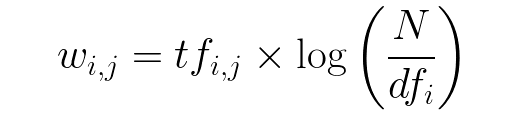
\includegraphics[scale=.5]{imagens/tfidf.png}}
	\caption{Equação TF-IDF}
	\label{fig}
	\end{figure}
     Onde:
\begin{itemize}
\item  Tf i,j é a quantidade de vezes que o palavra T aparece no texto u;
\item  N é a quantidade total de textos que compõem a base de entrada;
\item  df i é a quantidade de textos que contém a palavra T.
\end{itemize}

  Esse cálculo deve ser efetuado novamente com a entrada de novos documentos, pois a dimensão pode variar com entrada de n vos documentos e novos termos.
  
  
Foi utilizado a técnica de TF-IDF para criar nosso vetor de características considerando termos como palavras simples (\textit{onegrams}). Todos os termos foram gerados considerando cada documento como uma bag-of-words, sem considerar informações a respeito do contexto em que se encontra. Segundo Forman \cite{bagofwords}, o número de palavras candidatas a atributos excede o número de documentos em mais de uma ordem de magnitude, gerando matrizes esparsas e de alta dimensionalidade.
 
Para verificar quais candidatos são mais similares a uma determinada vaga, iremos aplicar a Similaridade do Cosseno pois é uma das medias mais utilizadas para definir similaridade entre dois documentos, pois favorece comparações do tipo zero-zero, sendo uma medida indicada aqui justamente,  pois estamos trabalhando com espaços de alta dimensionalidade e esparsos. O principio dessa métrica e medir o angulo formado por dois vetores como uma aproximação de similaridade. A similaridade do Cosseno é calculada pela equação da Figura 4:

	\begin{figure}[htbp]
	\centerline{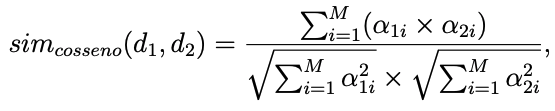
\includegraphics[scale=.4]{imagens/cosseno.png}}
	\caption{Equação Similaridade do Cosseno}
	\label{fig}
	\end{figure}

Essa medida retorna valores no intervalo [0,1]. Conforme o angulo entre os vetores diminui, o cosseno do ângulo se aproxima de 1, indicando que sua distancia é menor.

	\subsection{Sistemas de recomendação}
    	
 O objetivo dos Sistemas de Recomendação é o de retornar itens de possível interesse do usuário sem que o mesmo tenha que inserido nenhum dados em um formulário por exemplo, mas usando dados históricos. Esta tentativa de prever o que é mais adequado para um usuário é uma forma de tentar evitar a sobrecarga de informações.
    
 Esses sistemas vêm sendo implementados mediante o uso de diversas técnicas, que variam em função de aspectos como o objetivo a ser atingido e o tipo de item a ser recomendado.
    
Os Sistemas de Recomendação podem ser classificados em três tipos: filtragem colaborativa, baseada em conteúdo e híbridos \cite{sistema_recomendacao_3}. 

A Filtragem Baseada em Conteúdo parte do princípio de que os usuários tendem a interessar-se por itens similares aos que demonstraram interesse no passado. Assim é definida a similaridade entre os itens. Porém estabelecer esta similaridade entre itens pode não ser fácil em algumas situações \cite{sistema_recomendacao_content}. Para que seja estabelecida, por exemplo, a similaridade entre candidatos para uma vaga seria necessário que fossem identificados nos itens atributos a serem comparados (descrição da vaga, titulo da vaga, experiencias profissionais do candidato, por exemplo).

Na recomendação baseada em filtragem colaborativa o sistema realiza sua recomendação através da comparação dos usuários e a similaridade existente entre eles, ou seja, os objetos que são recomendados são os já utilizados anteriormente por usuários com características similares as de quem deseja a recomendação. Dessa forma, é encontrado um conjunto de usuários cujos gostos são semelhantes aos gostos do usuário em questão \cite{sistema_recomendacao_content}.
    
A abordagem da filtragem híbrida procura, basicamente, combinar os pontos fortes da filtragem colaborativa e filtragem baseada em conteúdo visando criar um sistema que possa melhor atender as necessidades do usuário. Essa abordagem é constituída de vantagens proporcionadas pela filtragem baseada em conteúdo e pela filtragem colaborativa, unindo o melhor das duas técnicas e eliminando as fraquezas de cada uma, conforme apresentado pela Figura 5.

\begin{figure}[htbp]
	\centerline{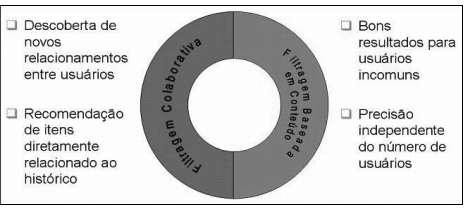
\includegraphics[scale=.5]{imagens/filtragem_hibrida.png}}
	\caption{ Filtragem Híbrida}
	\label{fig}
	\end{figure}

	
	\subsection{Redes Neurais}

As Redes Neurais Artificiais tiveram três importantes publicações iniciais, desenvolvidas por: McCulloch e Pitts (1943), Hebb (1949), e Rosemblatt (1958) \cite{perceptron}. Estas publicações introduziram o primeiro modelo de redes neurais simulando “máquinas”, o modelo básico de rede de auto-organização, e o modelo Perceptron de aprendizado supervisionado, respectivamente.
		
    Aprendizagem ou treinamento de rede neural artificial é equivalente a encontrar os valores de todos os pesos de tal forma que a saída desejada é gerada para a entrada correspondente, pode ser visto como a minimização da função de erro computada pela diferença entre a saída da rede e o desejado na saída de um conjunto de observações de treinamento \cite{redes_neurais_apredizagem}.
	
	Um neurônio artificial é um modelo matemático que recebe várias entradas, x1, x2, … xm e produz uma única saída, conforme ilustrado na Figura 6.
	
	\begin{figure}[htbp]
	\centerline{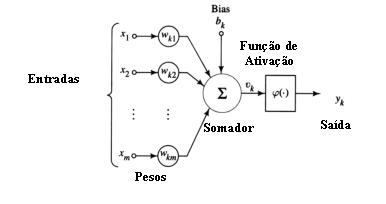
\includegraphics[scale=.7]{imagens/neuronio_artificial.jpg}}
	\caption{Modelo de Neurônio Artificial}
	\label{fig}
	\end{figure}
	
	No exemplo ilustrado na Figura 6, o neurônio possui n entradas: x1, x2, … xm. Rosenblatt propôs uma regra simples para calcular a saída. Ele introduziu pesos, w1, w2, …, números reais expressando a importância das respectivas entradas para a saída. A saída do neurônio, 0 ou 1, é determinada pela soma ponderada, menor ou maior do que algum valor limiar (\textit{threshold}) \cite{reuronio}. Assim como os pesos, o threshold é um número real que é um parâmetro do neurônio. 

    Esse modelo apresentado é um classificador linear e binário. Além disso, é usado na aprendizagem supervisionada e pode ser usado para classificar os dados de entrada fornecidos.
    
    Um único neurônio consegue resolver somente funções linearmente separáveis, mas como nosso modelo de dados tem características não linear, buscamos uma rede neural multicamadas.
    
    As redes neurais multicamadas são arquiteturas onde os neurônios são organizados em
    duas ou mais camadas de processamento, já que sempre vai existir pelo menos uma camada
    de entrada e uma camada de saída. 
    
    Uma arquitetura típica de rede neural artificial conhecida como Perceptron de Múltiplas Camadas (MLP) contém uma série de camadas, compostas de neurônios e suas conexões \cite{b14}. 
    
    A definição da arquitetura em redes MLP é um ponto muito relevante, a falta de conexões pode tornar a rede incapaz de resolver o problema de parâmetros ajustáveis, enquanto um excesso de conexões pode causar um ajuste excessivo dos dados de treinamento \cite{rede_neural}.
  
   \section{Avaliação de desempenho}
	 \subsection{Metodologia}

Objetivando criar um sistema de recomendação de candidatos para vagas, foi desenvolvido um modelo de rede neural capaz de classificar candidatos como aderentes ou não a determinas oportunidades de emprego.
Atendendo aos procedimentos metodológicos foram criadas, nesse estudo, as seguintes etapas:

\begin{enumerate}
\item Pesquisa bibliográfica sobre sistema de recomendação para candidatos \cite{artigo_referencia};
\item A base de dados foi fornecida pela Reachr Soluções Inovadoras em RH
\item Utilização das técnicas de mineração de dados para pré-processamento e aplicação de aprendizagem de máquina;
\item Aplicação da técnica de TF-IDF para criação da bag of words;
\item Analise descritiva dos dados gerados para identificação de anomalias;
\item Treinamento e criação de um modelo de rede neural utilizando uma cada escondida;
\end{enumerate}

Ao final dessas etapas, criou-se modelo capaz de informar se determinado candidato deve ou não ser indicado para determina vaga.

\subsection{Experimentos e resultados}

    Antes da aplicação da rede neural, foram utilizados algumas etapas de pré-processamento. 
    Durante a tarefa de limpeza, alguns registros foram removidos respeitando o seguinte critério: ter pelo menos dois campos preenchidos dos cinco existes no objeto.
    
    Foi realizado um processo de padronização no texto dos dos candidatos das vagas deixando conforme apresentado na Tabela III. Esse processo se fez necessário para evitar inconsistências na criação da nossa bag of words, que foi criada utilizando a técnica de TF-IDF \cite{tfidf3}.
    
    Primeiro selecionamos todas as vagas com seus respectivos candidatos aprovados e reprovados no processo seletivo para posteriormente aplicar a medida de similaridade do cosseno os mesmos. As combinações foram feitas em pares, conforme apresentado abaixo:
    
    \begin{enumerate}
    \item sim(Cargo profissional, Título vaga)
    \item sim(Atividade profissional, Descrição vaga)
    \item sim(curso técnico, Requisitos obrigatórios vaga)
    \item sim(Curso superior, Requisitos obrigatórios vaga)
    \item sim(Pós-graduação, Requisitos obrigatórios vaga)
    \item sim(Conhecimentos, Requisitos obrigatórios vaga)
    \item sim(Conhecimentos, Conhecimentos desejados vaga)
    \end{enumerate}

 Os seguintes termos serão utilizados respectivamente para referir as combinações mapeadas acima: sim-cargo, sim-descricao, sim-tecnico, sim-superior, sim-pos, sim-requisitos-obrigatorios e sim-conhecimentos-desejados.
    
O gráfico apresentado na Figura 7, mostra o valor médio das distâncias  de similaridade do cosseno para todos os registros comparando com as classes individuais.
      \begin{figure*}
    \centering
    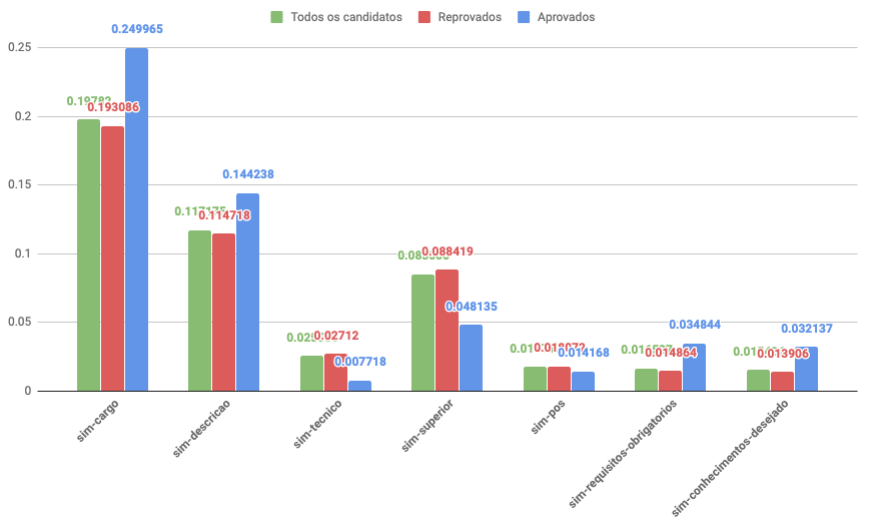
\includegraphics[scale=0.5]{imagens/barras.png}
    \caption{Valor médio das distâncias das similaridade do cosseno}
    \label{barras}
  	\end{figure*} 

 No diagrama de caixa ilustrado na Figura 8, podemos perceber que os candidatos aprovados (valor média 0.249965) tem um valor médio maior em relação aos reprovados(valor médio 0.193086). 
  \begin{figure*}
    \centering
    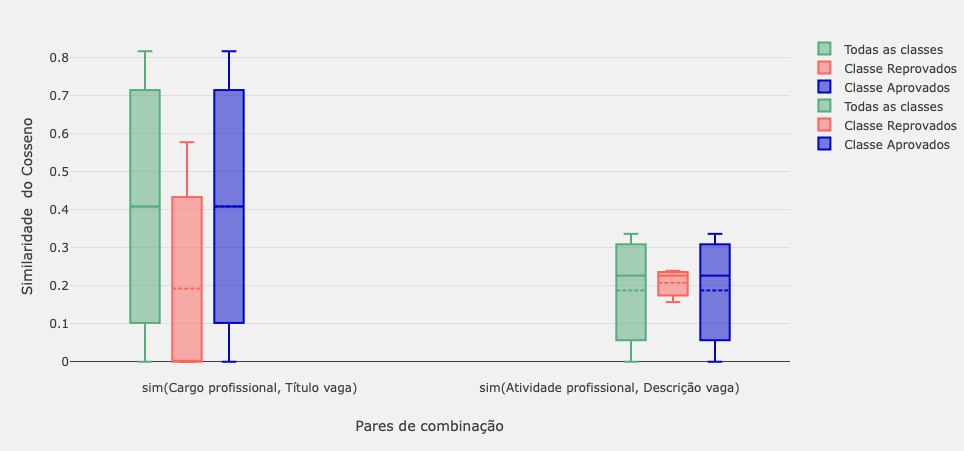
\includegraphics[scale=0.5]{imagens/grafico_dispersao.png}
    \caption{Dispersão de similaridade do cosseno das classes}
    \label{dispersao}
  \end{figure*} 

O próximo passo no experimento foi treinar uma rede neural que fosse capaz de classificar candidatos para tentar prever se os mesmos seriam ou não contratados para uma determinada vaga.
    A topologia de rede esta apresentada na figura Figura 9, e abaixo segue as configurações de criação do modelo preditivo. 
    
    Particularmente, não é possível resumir o processo de design das camadas ocultas com poucas regras. 
    
        \begin{figure}[htbp]
	\centerline{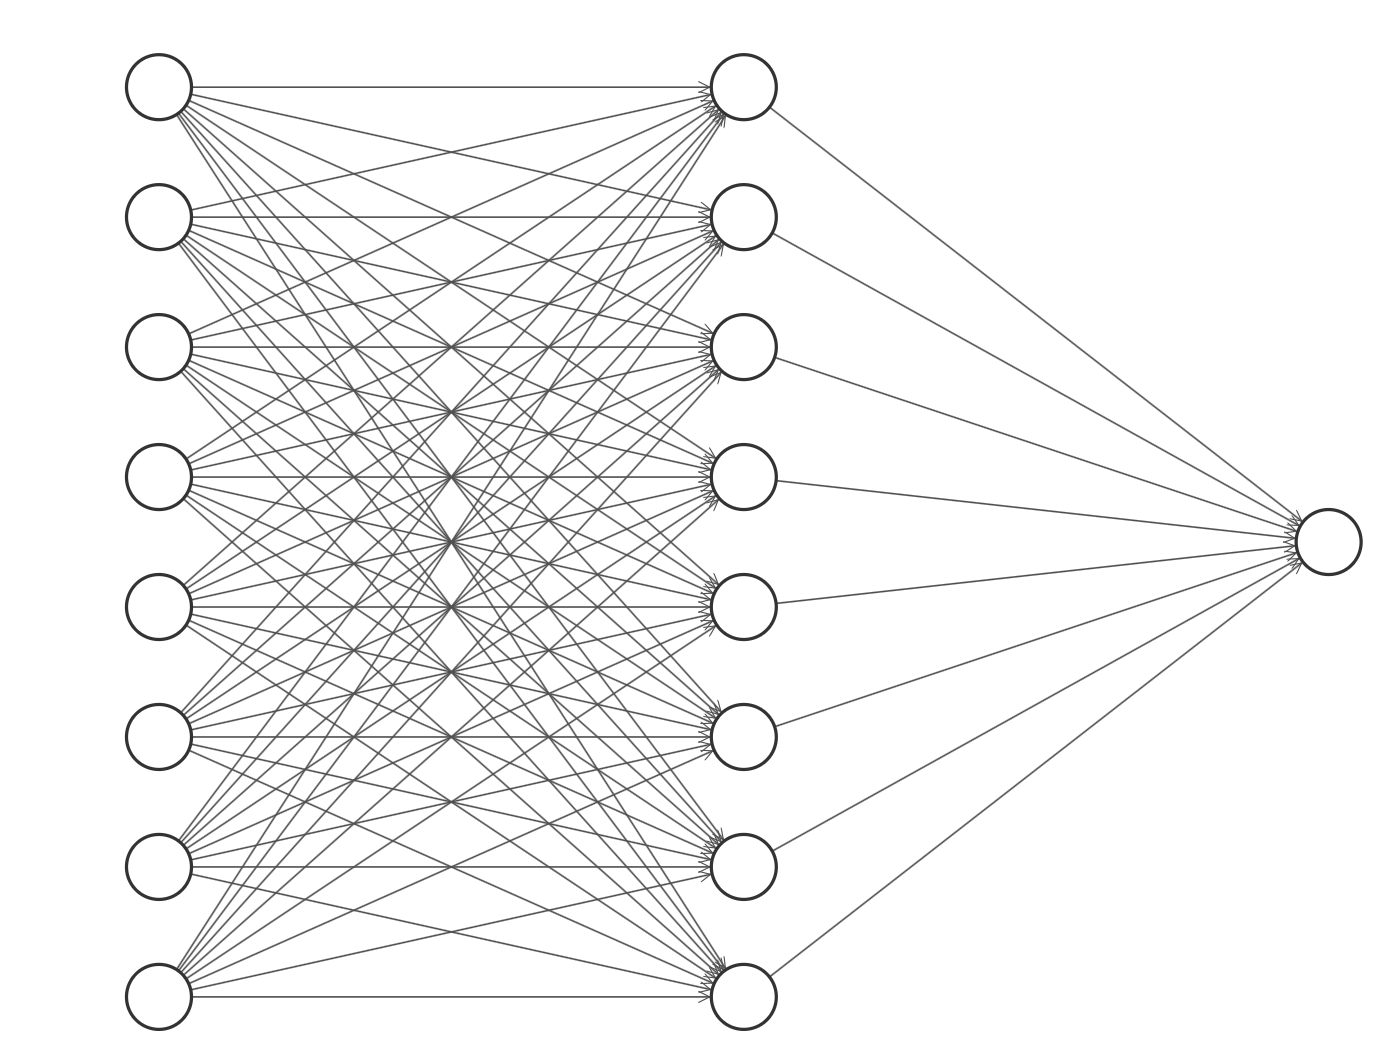
\includegraphics[scale=0.4]{imagens/topologia_rede_neural.png}}
	\caption{Topologia Rede Neural}
	
	\label{rede_neural}
	\end{figure}
    
   Dados e configurações utilizados na criação do modelo da rede neural:
    
     \begin{itemize}
    
    \item  Inicialização dos pesos: Aleatória;
    \item Taxa de aprendizado: 0,05;
    \item Número de iterações: 10.000;
    \item Camadas escondidas: 1;
    \item Número de neurônios na cada camada de entrada: 7;
    \item Número de neurônios na cada camada escondida: 7;
    \item Função de ativação: Relu;
    \item Número de neurônios na camada saída: ;
    \item Função de ativação na camada saída: Sigmoid;
    \end{itemize}
  
     
    \begin{table}[h]
	\caption{Matriz de confusão}
	\begin{center}
    \begin{tabular}{l | c | r }
    \hline
         \ & Aprovados  & Reprovados \\\hline
          Aprovados & 159  & 246    \\\hline
          Reprovados & 115 & 516    \\\hline
    \end{tabular}
    \end{center}
    \end{table}
     
Aplicamos as seguintes medidas  de avaliação para analisar a qualidade do modelo de classificação:
\begin{itemize}
\item Acurácia: corresponde a proporção entre os pontos segmentados corretamente, sendo eles regiões de interesse, com a soma destes mais os pontos definido falso positivos e falsos negativos;

     \[ACC = \frac{VP + VN}{VP+VN+FP+FN} = 65,15\%\]

\item Precisão: taxa com que todos os exemplos classificados como positivos são realmente positivos. Nenhum exemplo negativo é incluído.

    \[PRE = \frac{VP}{VP+FP} = 58,02\%\]

\item  Revocação: porcentagem de exemplos positivos classificados como positivos;

    \[REV = \frac{VP}{VP+FN} = 39,55\%\]
\end{itemize}

    
    \subsection{Análise dos resultados}
	   %porques%

	 Ao analisarmos o gráfico da Figura 7 podemos verificar que candidatos aprovados em processos seletivos tiveram em média uma similaridade maior que os reprovados (sim-cargo, sim-descricao, sim-requisitos-obrigatorios e sim-conhecimentos-desejados). 
     O mesmo comportamento aparece no gráfico de dispersão Figura 8. Com isso, podemos chegar a conclusão que a experiência profissional e as atividades exercidas anteriormente tiveram grande influência na tomada de decisão dos recrutadores.
     Nosso modelo não teve uma grande acurácia conforme apresentado na Tabela IV. Isso se deve a qualidade dos dados, pois muitos dos mesmos estavam vazios . Devido a incompletude, grande parte dos candidatos aprovados não puderam ser utilizados para treinar nosso modelo, deixando as classes desbalanceadas. Isso fica evidente quando olhamos os numero de revocação e precisão.
	   
\section*{Conclusão perspectivas futuras}

    Motivado pelo potencial dos sistemas de recomendação estudamos como criar modelos de seleção de candidatos de forma automática. A proposta aqui é utilizar uma rede neural para aprender o que é relevante para empresas no quesito de analise de currículo.
    O volume de currículos dificulta o processo de busca e filtragem de informações, com isso, sistemas de recomendação se tornaram importantes e necessários para auxiliar usuários.
    Considerando-se que o objetivo principal deste trabalho era criar um classificador para predizer se um candidato deve ou não ser recomendados para vaga, podemos considerar como atingido.
    Para os próximos experimentos, irei utilizar os processos descritos aqui para aplicar em outros algoritmos de aprendizagem de máquina buscando melhores resultados.

\begin{thebibliography}

\bibitem{artigo_referencia} F. Borisyuk, K. Kenthapadi, D. Stein, and B. Zhao. CaSMoS: A framework for
learning candidate selection models over structured queries and documents. In
KDD, 2016

\bibitem{mineracao} LAROSE, D. T. Discovering Knowledge in Data: An Introduction to Data Mining.
John Wiley and Sons, Inc, 2005.

\bibitem{mineracao_nunes} CASTRO, Leandro Nunes de; FERRARI, Daniel Gomes. Introdução à mineração de
dados: conceitos básicos, algoritmos e aplicações. São Paulo: Saraiva, 2016.

\bibitem{kdd} FAYYAD, U; PIATETSKY-SHAPIRO, G; SMYTH, P. From Data Mining to Knowledge Discovery in Databases. American Association for Artificial Intelligence, 1996.

\bibitem{mineracao_conceitos_tecnicas} HAN, J; KAMBER, M. Data Mining: Concepts and Techniques. Elsevier, 2006.

\bibitem {tokenizacao} Terry Padgett, Angelo Maniquis, Mark Hoffman, Will Miller, and Jennifer Lautenschlager. A semantic visualization tool for knowledge discovery and exploration in a
collaborative environment. In International Conference on Intelligence Analysis: The
Office of the Assistant Director of Central Intelligence, 2005. 5 

\bibitem{tfidf} Djoerd Hiemstra. A probabilistic justification for using tf$\times$ idf term weighting
in information retrieval. International Journal on Digital Libraries, 3(2):131–139,
2000. 6

\bibitem{tfidf2} Juan Ramos. Using TF-IDF to determine word relevance in document queries.
In Proceedings of the first instructional conference on machine learning, 2003. 7

\bibitem{tfidf1} David M. Blei, Andrew Y. Ng, and Michael I. Jordan. Latent dirichlet allocation.
the Journal of machine Learning research, 3:993–1022, 2003. 7

\bibitem{tfidf3} Salton, G.; Buckley, C.. Term-weighting approaches in automatic text retrieval.
Information Processing and Management – Cornell University, Ithaca, 1988.

\bibitem {redes_neurais_apredizagem} M. Ettaouil and Y. Ghanou, “Neural architectures optimization and Genetic algorithms”, Wseas Transactions On Computer, Issue 3, Volume 8, 2009, pp. 526-537. 

\bibitem{reuronio} Rosenblatt, “The Perceptron: A Theory of Statistical Separability in Cognitive Systems”, Cornell Aeronautical Laboratory, Report No. VG1196-G-1, January, 1958. 

\bibitem{b5} Ramchoun H, Amine M, Idrissi J, Ghanou Y, Ettaouil M. Multilayer Perceptron: Architecture Optimization and Training. International Journal of Interactive Multimedia and Artificial Intelligence. 2016;4(1):26–30.

\bibitem{bagofwords}FORMAN, G., 2003, “An extensive empirical study of feature selection metrics for
text classification”, The Journal of Machine Learning Research, 3, pp. 1289–
1305.

\bibitem{perceptron} Rosenblatt, “The Perceptron: A Theory of Statistical Separability in Cognitive Systems”, Cornell Aeronautical Laboratory, Report No. VG1196-G-1, January, 1958. 

\bibitem{sistema_recomendacao_content} J. M. Pazzani. A Framework for Collaborative, Content- Based and Demographic Filtering. Artificial Intelligence Review, 13(5-6). páginas 393–408, 1999.

\bibitem{sistema_recomendacao_content2} U. Shardanand, P. Maes. Social Information Filtering: Algorithms for Automating “Word of Mouth”. In: ACM CHI’95 Conference on Human Factor in Computing Systems, Proceedings, (1). páginas 210–217, 1995.

\bibitem{sistema_recomendacao_3} Adomavicius, G. & Tuzhilin, A. (2005). Toward the Next Generation of Recommender
Systems: A Survey of the State-of-the-Art and Possible Extensions. In IEEE
Transactions On Knowledge and Data Engineering, vol. 17, no. 6, p. 734–749.


\bibitem{b4} Salchenberger LM, Cinar E, Lash NA. Neural networks: A new tool for predicting thrift failures. Decision Sciences. 1992;23(4):899–916

\bibitem{b14} S. Haykin, Redes Neurais: Princípios e prática, Bookman, 2. ed., 2001.

\bibitem {rede_neural} T.B Ludermir “Hybrid Optimization Algorithm for the Definition of MLP Neural Network Architectures and Weights” Proceedings of the Fifth International Conference on Hybrid Intelligent Systems (HIS’05) 0-7695- 2457-5/05 20.00 2005 IEEE.





\end{thebibliography}
\end{document}